\documentclass[12pt]{article}
\usepackage[utf8]{inputenc}
\usepackage{graphicx}
\usepackage{cite}
\usepackage{enumerate}
\usepackage[LAE,T1]{fontenc}
\usepackage[arabic,UKenglish]{babel}

% Keywords command
\providecommand{\keywords}[1]
{
  \small    
  \textbf{\textit{Keywords---}} #1
}

\begin{document}

  \title{\Large Nuqud: A Decentralized Digital Cryptocurrency}
  \author{Jaâfar Moussaid\\ jafar@mussa.id\\ www.nuqud.org}
  \date{July 20, 2020}

  \maketitle
  \thispagestyle{empty}

\begin{abstract}
The future of finance is decentralized. Where transactions are direct online peer-to-peer, securely and without the need for a trusted third party. The market continues to grow, bringing with it more \emph{freedom}. Nuqud is part of this decentralized finance movement. It combines stablecoin and digital cryptocurrency properties. Its pre-mined fixed supply is pegged to a minimum value, without a maximum. Initially, the value of Nuqud depends on that of gold. Then it will depend entirely on the market. As Nuqud gains popularity, it gains utility as a form of digital cryptocurrency. It exists as a smart contract on the Ethereum blockchain, secured by millions of computers worldwide. Decentralized exchanges allow online direct peer-to-peer cryptocurrency transactions. Nuqud will be listed on many decentralized finance protocols. Decentralized exchange protocol facilitates automated transactions between cryptocurrency tokens on the Ethereum blockchain. Nuqud is an open-source project, released under MIT license. You can feel free to contribute. We are witnessing a revolution, we are at the beginning of the post-bitcoin era. The number of people adopting this new version of finance continues to increase. Cryptocurrency volatility keeps decreasing. In the near future, they can be fully used in our daily life. Reserve your seats, the moon is our destination.
\end{abstract}
\keywords{Nuqud, Decentralized, Cryptocurrency, Blockchain, Ethereum, Finance, DeFi, Freedom}

\section{Introduction}\label{sec:int}

The global telecommunication revolution has enabled the emergence of a new connected version of traditional finance, in which banks and other firms utilized computer and network technology for payments and recordkeeping. In this version, traditional financial institutions act as trusted third parties to process electronic payments. These institutions apply a mediation cost, increasing the transaction cost, limiting the minimum transaction size. They also apply the "date de valeur", a transaction made on Thursday would be credited on Monday. Further the possibility of lost transactions. Certain methods of fraud are accepted as inevitable. These costs, delays and uncertainties can be avoided by using physical currency. Hence the need for a mechanism to make payments over a communication channel without a trusted party.

Decentralization consists of a transfer of power from the center to autonomous entities, linked to each other by peer-to-peer rules. The Blockchain is a decentralized system, made up of databases, called \emph{blocks}, distributed across different physical locations, linked together by a digital signatures \emph{chain}, governed by proof-of-work \cite{nakamoto2008bitcoin}. Bitcoin (BTC) is the first decentralized digital cryptocurrency that can be sent from user to user on the peer-to-peer bitcoin network without the need for intermediaries. It was invented in 2008 by an unknown person or group of people using the name Satoshi Nakamoto. Transactions are verified by network symmetric units, called \emph{nodes}, each one has the same ability to send, receive and calculate as the other nodes in its network, linked together using cryptography. All transactions are recorded in a public digital \emph{ledger} known as blockchain. After Bitcoin, several altcoins appeared. They are based on the same technology as Bitcoin, using a consensus mechanism to produce blocks or validate transactions. Their added value is to provide new or additional capabilities, such as smart contracts (e.g. Ethereum) or low price volatility (e.g. stablecoins).

In French the word “defi” means challenge. Decentralized finance (DeFi) is a blockchain-based form of finance that utilizes smart contracts. DeFi platforms allow people to lend or borrow funds from others, trade cryptocurrencies, without the need for a trusted third party. Nuqud project will be our "challenge" to be part of the DeFi market.

\section{Design}

Nuqud (in Arabic: \foreignlanguage{arabic}{\textRL{نقود}}, meaning \emph{money}) is an open-source decentralized digital cryptocurrency project \cite{nuqud2021repository}, based on the OpenZeppelin framework, released under the MIT license. OpenZeppelin is an open-source framework to build secure smart contracts. The framework provides a complete suite of security products and audit services to build, manage, and inspect all aspects of software development and operations for decentralized applications. The MIT licence gives you the ability to consult, modify and redistribute the source code. Nuqud's open-source design confirms our desire to assert the value of freedom. All other products developed as part of this project will be open-source. Bitcoin was not developed to enrich us, but above all to preserve our freedom.

\subsection{Units and divisibility}
The ticker symbol used to represent nuqud is NQD. Its character is  {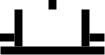
\includegraphics[width=.03\linewidth]{n.png}}. Small amounts of nuqud used as alternative units are millinuqud (mNQD) and naqd (in Arabic: \foreignlanguage{arabic}{\textRL{نقد}}, \emph{singular} of money). A naqd is the smallest amount within nuqud representing $1/10^{18}$ nuquds, one quintillionth of a nuqud. A millinuqud equals 1/1000 nuquds; one-thousandth of a nuqud or one quadrillion naqds.

\subsection{Concept}
Mining is the process through which cryptocurrency transactions are gathered, verified and recorded. The essential role of miners is to maintain the integrity of the network and introduce new coins into the system. This process is energetically very expensive. Against global warming, it is essential to reduce our energy consumption, to use it more efficiently and to diversify our sources, by replacing fossil fuels with renewable energies. The pre-mining of tokens permits us to partially reduce our energy consumption. Nuqud is pre-mined to a fixed supply of 21,000,000 tokens pegged to a minimum of  1.00 $\mu$g of gold per token, without a maximum value (Figure 1).
\begin{figure}[!h]
  \centering
  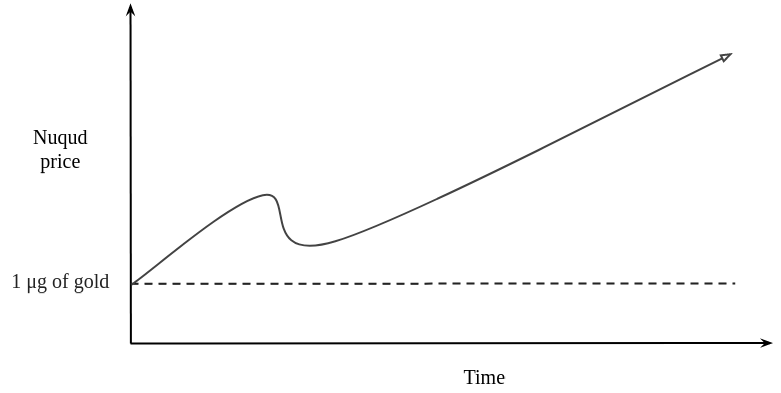
\includegraphics[width=.78\linewidth]{figure1}
  \caption{To the Moon!}
  \label{fig:f1}
\end{figure}

When \emph{demand} is greater than \emph{supply}, the \emph{value} may increase above the initial peg-value of 1.00 $\mu$g of gold.  For example, if 1000 people each want 1000 Nuquds, the fair market value of Nuqud is 1.00 $\mu$g each. If 2000 people each want 1000 Nuquds, the fair market value of Nuqud rises to 2.00 $\mu$g, thereby increasing the market capitalization. Over time, the price of Nuqud may reach 1.00 mg, 1.00 g, or even higher.

\subsection{Properties}
Nuqud has its unique properties, where stablecoin and digital cryptocurrency are combined.  We start with a stable value, then we move towards the moon without limit. Nuqud's smart contract is written in Solidity \cite{nqd2021etherscan} (Table 1):
\begin{table}[!h]
  \begin{center}
    \label{tab:t1}
    \begin{tabular}{|l|r|}
      \hline
      Total Supply &  21,000,000\\
      \hline
      Name  &  Nuqud\\
      \hline
      Symbol &  NQD\\
      \hline
      Decimals & 18\\
      \hline
    \end{tabular}
    \caption{Smart Contract Characteristics}
  \end{center}
\end{table}

Solidity is an object-oriented programming language for writing smart contracts. It is used for implementing smart contracts on various blockchains, platforms, most notably, Ethereum (ETH). The programs compiled by Solidity are intended to be run on Ethereum Virtual Machine (EVM). The Nuqud smart contract characteristics, once deployed on the blockchain, can never be changed again. This guarantees more trust between the users of the contract.

\begin{enumerate}[(a)]
\item Fixed limited supply:\\
  Nuqud has a fixed supply of 21,000,000 tokens total. No more can ever be created, guaranteed by code. It is \emph{deflationary} by nature. It begins with a peg of 1.00 $\mu$g of gold per token, and its value increases over time with scarcity. Nuqud is “scarce” in the sense that it is available in very low numbers.\\
  {}\\
  “Scarcity is the fundamental starting point of all economics, and its most important implication is the notion that everything has an opportunity cost.”
 —Saifedean Ammous \cite{ammous2018bitcoin}\\
 {}\\
Market capitalization is equal to the token price multiplied by the number of tokens outstanding. With a peg-value of 1.00 $\mu$g of gold, Nuqud starts with a minimum market capitalization. Beyond its minimum value, the total market capitalization depends totally on supply and demand. Over the past years, digital cryptocurrencies have performed very well.\\ 
{}\\
For holders of Nuqud, there is an unlimited upside. Unlike traditional stablecoins (pegged to 1 Token = 1.00 g of gold, e.g. Digix), Nuqud has a fixed supply and therefore has an unbound maximum. As Nuqud gains popularity and circulation, total market capitalization could potentially reach higher values being worth as much as \$10 million or \$100 million theoretically. The moon is the limit.

\item Utility:\\
As Nuqud gains popularity amongst more and more people, it gains \emph{usage} and \emph{acceptance} as a form of digital cryptocurrency spreading exponentially through word of mouth. Nuqud can be used as both a store of value and a means of transaction. Nuqud’s limited supply makes it especially ideal as a store of value with unlimited upside. It can be transferred in fractional amounts (up to 18 decimals), allowing it to be used for microtransactions as well.\\
{}\\
A cryptocurrency gets its utility as a mode of payment due to two key factors: (i) Transaction Costs, to transfer a cryptocurrency is near minimal as the number of parties involved is technically only two; (ii) Transaction Time, it’s more like a cash transaction done digitally. Blockchain utilizes \emph{public key} cryptography to allow secure value exchange over an open unsecured network. Each cryptocurrency \emph{wallet} is identified on the blockchain by a public key. Some wallets (e.g MetaMask) do not require KYC\footnote{KYC (Know-Your-Customer), the Financial Action Task Force (FATF) has published new draft guidance that could require decentralized finance (DeFi) platforms to find a way to implement KYC rules. This risks affecting our right to anonymity.} verification. Therefore, Blockchain's anonymity allows for more confidentiality and preserves our privacy.

\item Security:\\
Nuqud exists as an ERC-20\footnote{ERC-20 (Ethereum Request for Comments 20) Token Standard allows for fungible tokens on the Ethereum blockchain.} smart contract on the Ethereum blockchain \cite{oliva2020exploratory}. As a decentralized currency secured by millions of computers worldwide. In the blockchain, we apply a \emph{consensus mechanism} twice: (i) accept a new block on the blockchain; (ii) validate the reliability of the nodes, information unknown to the majority is therefore refused. The blockchain is designed so that it can preserve the data stored in it and prevent it from being modified, meaning that when a piece of information is stored in the blockchain, this information cannot be modified later \cite{zheng2017overview}\cite{tsankov2018securify}. Blockchain is \emph{secure} by design and is an example of distributed computer system distribution with high Byzantine fault tolerance \cite{kirrmann2005fault}. The blockchain thus allows a decentralized consensus system.\\
{}\\
A consensus mechanism in a cryptoeconomic system also helps prevent certain kinds of economic attacks. In theory, an attacker can compromise consensus by controlling 51\% of the network. Consensus mechanisms are designed to make this "51\% attack" unfeasible. Different mechanisms are engineered to solve this security problem differently. There are two types of consensus mechanisms: (i) proof-of-work (PoW), used currently by Bitcoin (BTC), is done by miners, who compete to create new blocks full of processed transactions. The winner shares the new block with the rest of the network and earns some freshly minted coins. The race is won by whoever computer can solve a math puzzle fastest – this produces the cryptographic link between the current block and the block that went before. Solving this puzzle is the work of "proof-of-work". (ii) Proof-of-stake (PoS), Ethereum has plans to upgrade to a PoS consensus protocol. PoS is done by validators who have staked ETH to participate in the system. A validator is chosen at random to create new blocks, share them with the network and earn rewards. Instead of needing to do intense computational work, you simply need to have staked your ETH in the network. This is what incentivises healthy network behaviour. The network is kept secure by the fact that you'd need 51\% of the network's computing power to defraud the chain. This would require such huge investments in equipment and energy, you are likely to spend more than you had gain.
\end{enumerate}

\subsection{Exchange}
Decentralized exchanges (DEX) allow direct peer-to-peer cryptocurrency transactions to take place online securely and without the need for a trusted third party. In the DeFi ecosystem, instead of the traditional order book, we use an automated market maker (AMM), a type of DEX protocol that relies on a mathematical formula to price assets. This formula can vary with each protocol. Some use a simple formula like Uniswap, while Curve, Balancer and others use more complicated ones. They work with liquidity pools (LP), each LP consists of a pair of tokens (X, Y).  For example, Uniswap uses x * y = k, where x is the amount of one token in the liquidity pool, and y is the amount of the other. In this formula, k is a fixed constant, meaning the pool’s total liquidity.

Nuqud is listed on Uniswap \cite{uniswap2020protocol}, the protocol facilitates automated transactions between cryptocurrency tokens on the Ethereum blockchain through the use of smart contracts. Nuqud would then be listed on other exchanges. Some exchanges will list Nuqud due to its popularity, others will require a certain level of market capitalization. Create a digital currency wallet (e.g. MetaMask). Feed your wallet with coins (Ethereum, USDC, or others). Connect to your chosen exchange (e.g. Uniswap) and trade for Nuqud (\$NQD).

At the start, the peg-value will be defined using a liquidity pool. This is the minimum value we will buy with it. Anyone can become a \emph{market maker} on an exchange, by providing liquidity to a liquidity pool, and earn fees for providing liquidity \cite{liquidity2021pools}. Anytime you can sell your LP-Tokens and redeem your position.

\section{Conclusion}
In today’s market, blockchain technology enables individuals to trade directly with each other. Without the need for a trusted third party. We are witnessing a revolution, the blockchain will forever change the world of finance. There is a pre-bitcoin and post-bitcoin era (Table 2).
\begin{table}[!h]
  \begin{center}
    \label{tab:t2}
    \begin{tabular}{|l|l|}
      \hline
      \textbf{Pre-bitcoin} &  \textbf{Post-bitcoin}\\
      \hline
      centralized  &  decentralized\\
      \hline
      client–server &  peer-to-peer\\
      \hline
      trusted third party & proof-of-work\\
      \hline
      printing & mining\\
      \hline
      order book & automated market maker\\
      \hline
      trader & market maker\\
      \hline
      inflation & deflation\\
      \hline
    \end{tabular}
    \caption{Pre-bitcoin and post-bitcoin era}
  \end{center}
\end{table}

Our language will change, we will be more and more familiar with the new vocabulary, we will not talk about the same thing anymore. If we keep our money in fiat format - at best - it will keep its value stable until next year. However, the inflation during the current year will represent a loss of value. For example, If you can buy some products in today's market for \$100, after a year, if the average inflation value is 3\%, the same group of products is worth 3\% more. In other words, we need \$103 to buy the same thing, which means the \$100 of yesterday has become \$97 today. Inflation, therefore, represents a loss of value. The value of inflation depends on each market. Let chose the case of the United States \cite{usd2020inflation}.

\clearpage

\begin{figure}[!h]
  \centering
  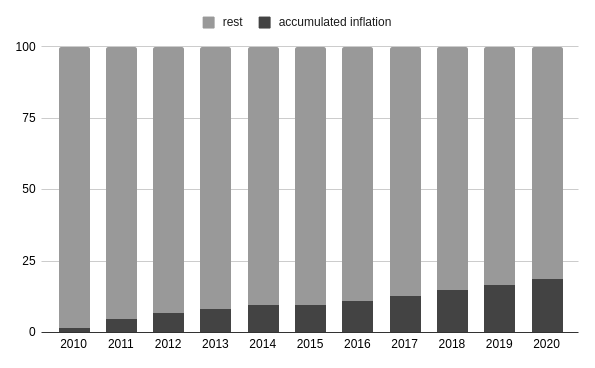
\includegraphics[width=.8\linewidth]{figure2}
  \caption{Accumulated inflation}
  \label{fig:f2}
\end{figure}

“We now have a tiger by the tail: how long can this inflation continue? If the tiger (of inflation) is freed he will eat us up; yet if he runs faster and faster while we desperately hold on, we are still finished! I'm glad I won't be here to see the final outcome.”\\
—Friedrich Hayek \cite{hayek1971tiger}\\
{}

For inflation values between 0.12\% and 3.14\%, from 2010 to 2020, the accumulated inflation value is 18.88\%. For example, someone who kept \$100 in their account in 2010, their \$100 is worth \$81.12 in 2020, in the same market. Let suppose this same person chooses to keep their \$100 in their bitcoin wallet, by 2020 their wealth has exceeded \$1 billion. Yes, this is an \emph{early adopter} case and it will not always be the case, however bitcoin and altcoins will behave like any other commodity in the market; no more inflation, just deflation.

This new version of finance ensures more freedom, security, rigor and anonymity. Cryptocurrency volatility keeps decreasing. Today bitcoin's (BTC) volatility is about 70\% (Figure 3), against 5\% for the US dollar \cite{usd2020volatility}.
\clearpage
\begin{figure}[!h]
  \centering
  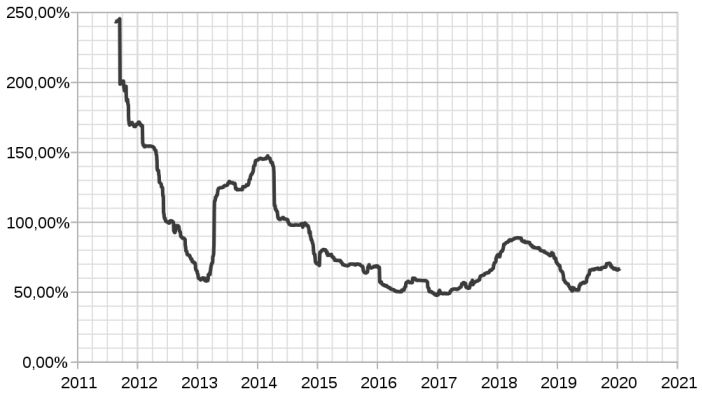
\includegraphics[width=.8\linewidth]{figure31}
  \caption{Accumulated inflation}
  \label{fig:f2}
\end{figure}

Even if in the future we would be in values close to those of stablecoins, the value of the cryptocurrency will evolve like all other commodities in the market. In this case, cryptocurrency volatility will be equal to the mean volatility of a stablecoin plus the average value of inflation. “Any person who owns Bitcoin achieves a degree of economic freedom which was not possible before its invention. Bitcoin holders can send large amounts of value across the planet without having to ask for the permission of anyone. Bitcoin's value is not reliant on anything physical anywhere in the world and thus can never be completely impeded, destroyed, or confiscated by any of the physical forces of the political or criminal worlds.” —Saifedean Ammous \cite{ammous2018bitcoin}

In the near future, cryptocurrency will be fully used in our daily life. Hence the need for various blockchain projects to meet our needs and ensure our freedom. Nuqud is an open-source project \cite{nuqud2021repository}, released under MIT license. You can feel free to contribute. We are at the beginning of this project. After that, we will develop other products to facilitate the use of cryptocurrencies. It is far easier to move around with a Nuqud private key than with a hoard of gold, and far easier to send it across the world without having to risk it getting stolen or confiscated. The future market is a fully decentralized one. We are moving to the Moon.

\bibliographystyle{ieeetr}
\bibliography{references}

\end{document}
